\documentclass[11pt,spanish]{article} % Idioma
\usepackage{babel}
\usepackage[T1]{fontenc}
\usepackage{textcomp, verbatim} % \begin{comment}
\usepackage[utf8]{inputenc} % Permite acentos

\usepackage{wrapfig} % Imagenes %\graphicspath{ {./imagenes/} }
\usepackage[left=2.75cm,top=2.5cm,right=2cm,bottom=2.5cm]{geometry} % Márgenes
\usepackage{amssymb, amsmath, amscd, amsfonts, amsthm, mathrsfs } % Símbolos matemáticos
\usepackage{cancel} % Cancelar expresiones
\usepackage{multirow, multicol, tabularx, booktabs, longtable} % Tablas
\usepackage{fancyhdr, fncychap} % Encabezados
\usepackage{algpseudocode, algorithmicx, algorithm} % Pseudo-código	
\usepackage{bbding} % Símbolos
\usepackage{enumitem} % Enumerados a), b), c)... usando \begin{enumerate}[label=\alph*)]
\usepackage{graphicx, xcolor, color, pstricks} % Gráficos --TikZ-- 
% http://www.texample.net/tikz/examples/
\usepackage[hidelinks]{hyperref}  % Enlaces
\usepackage{verbatim} % Comentarios largos \begin{comment}
\usepackage{rotating} % \begin{rotate}{30}
\usepackage[all]{xy} % Diagramas
\usepackage{xparse} % Entornos
\usepackage{listings}
\usepackage{float} %Permite fijar la posición de una imagen en el texto poniendo {figure}[H] 
 
\definecolor{codegreen}{rgb}{0,0.6,0}
\definecolor{codegray}{rgb}{0.5,0.5,0.5}
\definecolor{codepurple}{rgb}{0.58,0,0.82}
\definecolor{backcolour}{rgb}{0.95,0.95,0.92}



\lstdefinestyle{mystyle}{
	backgroundcolor=\color{backcolour},   
	commentstyle=\color{codegreen},
	keywordstyle=\color{magenta},
	numberstyle=\tiny\color{codegray},
	stringstyle=\color{codepurple},
	basicstyle=\footnotesize,
	breakatwhitespace=false,         
	breaklines=true,                 
	captionpos=b,                    
	keepspaces=true,                 
	numbers=left,                    
	numbersep=5pt,                  
	showspaces=false,                
	showstringspaces=false,
	showtabs=false,                  
	tabsize=2
}
\lstset{style=mystyle}



% Comandos
\newcommand{\docdate}{}
\newcommand{\subject}{}
\newcommand{\docauthor}{Rubén Morales Pérez}
\newcommand{\docemail}{srmorales@correo.ugr.es}

\newcommand{\N}{\mathbb{N}}
\newcommand{\Q}{\mathbb{Q}}
\newcommand{\C}{\mathbb{C}}
\newcommand{\R}{\mathbb{R}}
\newcommand{\Z}{\mathbb{Z}}


\linespread{1.1}                  % Espacio entre líneas.
\setlength\parindent{0pt}         % Indentación para párrafo.

\usepackage[pages=some]{background}
% configuración
\backgroundsetup{
 scale=1, %escala de la imagen, es recomendable que sea del mismo tamaño que el pdf
 color=black, %fondo a usar para transparencia
 opacity=0.2, %nivel de transparencia
 angle=0, %en caso de querer una rotación
 contents={%
  
\includegraphics[width=\paperwidth]{ikaruslogo.jpg}} %nombre de la imagen a utilizar como fondo
 }%

\title{Proyecto IX Desafío Tecnológico ETSIIT\\
		Dron para monitorización de agricultura y silvicultura }
\author{Ikarus Ants}
\date{\today}

% % % % % % % % % % % % % % % % % % % % % % % % % % % % % % % % %
%					 Inicio del documento
% % % % % % % % % % % % % % % % % % % % % % % % % % % % % % % % %
\begin{document}
\BgThispage
\maketitle
\tableofcontents % Generando el indice
\newpage
\setlength\parindent{0pt} % Quitamos la sangría



\section{¿Qué problema intenta resolver su proyecto?}

El objetivo de este proyecto es permitir el análisis de cultivos y/o zonas forestales mediante fotografías con drones aéreos, prescindiendo de la imagen por satélite. Estos permitirán cubrir con mayor detalle (en resolución y cantidad de datos) una zona pequeña o mediana de un entorno natural o de cultivo. 
En el ámbito de cultivo se hará especial énfasis en el cultivo del olivo mediante un análisis de los parámetros del mismo, permitiendo solucionar algunos problemas presentes que perjudican a los productores como la detección a tiempo de enfermedades y plagas. Dicha detección permitiría aumentar el rendimiento de las cosechas y asegurar un estado de salud óptimo en dicha plantación. 

\

En adición, se quiere extender su funcionalidad para solucionar aspectos de importancia en el control forestal como la prevención de incendios, detección de puntos calientes de un incendio, presencia de humo y su posible propagación según la dirección del viento.

\

Se abordarán diversas actividades como la detección de plásticos, mapeo del bosque, estudio de su biodiversidad y su posible aplicación a agricultura de precisión y una silvicultura de precisión que permitiría una explotación más controlada de recursos forestales.


\subsection{¿A qué clientes va destinado?}
Particulares y empresas agrarias de cualquier cultivo, en particular del olivar.
Empresas de gestión de reservas naturales.
Empresas de investigación científica, en especial, en ciencias naturales y biología.


\subsection{¿Qué productos/empresas hacen algo similar?}
\textit{Cegadrone}. Empresa española con sede en Madrid especializado en un gran campo de aplicaciones de drones, siendo dos de sus servicios en el ámbito de agricultura y control forestal. 

\

\textit{Aeromedia}. Empresa española con sede en Málaga, Alicantes y Burgos. Se centra en servicios agro-forestales y en prevención de incendios abordando el problema principalmente con la medición de estados de cortafuegos, informes de la causas de incendios o reconstrucciones de incendios, análisis y valoración de daños.

\

\textit{Recdron}. Empresa española con sede en Murcia y Granada centrada en producción audiovisual con un servicio secundario de agricultura de precisión. Ofrece vuelos periódicos a fincas para dar recomendaciones para mejorar los cultivos según los datos recogidos.  

\

\textit{Zenit drones}. Empresa de drones de Motril centrado en agricultura de precisión, inspección industrial, termografía y audiovisual.

\

\textit{Tvant}. Empresa de drones de Córdoba que da servicio a toda Andalucía. Se centran en el sector de la agricultura de precisión. Precio variable según la tarea a solucionar.

\subsection{¿En qué se diferencian esos productos/empresas de su propuesta?}
Se ofrece un servicio periódico asequible sin requerir una gran inversión inicial. 
Instalación de una estación en el terreno, cuyo papel es la recarga de los drones y transmisión de datos a la nube.
Vuelo autónomo, puede funcionar de forma autónoma sin necesidad de personal especializado.
Interfaz fácil y accesible desde una aplicación web.
Recolección y tratamiento de datos, que informan al cliente del estado de su terreno y cultivos.

\subsection{¿Cuáles son los costes más importantes por fabricación de cada unidad, mantenimiento e instalación?}

Dron con capacidad de vuelo autónomo.
Sistema de cámara multiespectral y térmica y unidad de procesamiento de datos.
Base del dron para recarga automática, comunicación con servidores y recarga solar.
Coste adicional: infraestructura de red para la comunicación y monitorización.

\subsection{¿Cómo obtendrá beneficios del producto (por adquisición de cada unidad, por mantenimiento, por instalación, por análisis de datos que genera...)?}
Proveemos un servicio, nuestra empresa se reserva el derecho de propiedad del sistema autónomo aunque se encuentre en la instalación de cultivo del cliente. La empresa realiza la instalación y mantenimiento activo el servicio mediante un coste mensual, trimestral o anuales asequible.

\subsection{Business Model Canvas}
\begin{figure}[H]
	\centering
	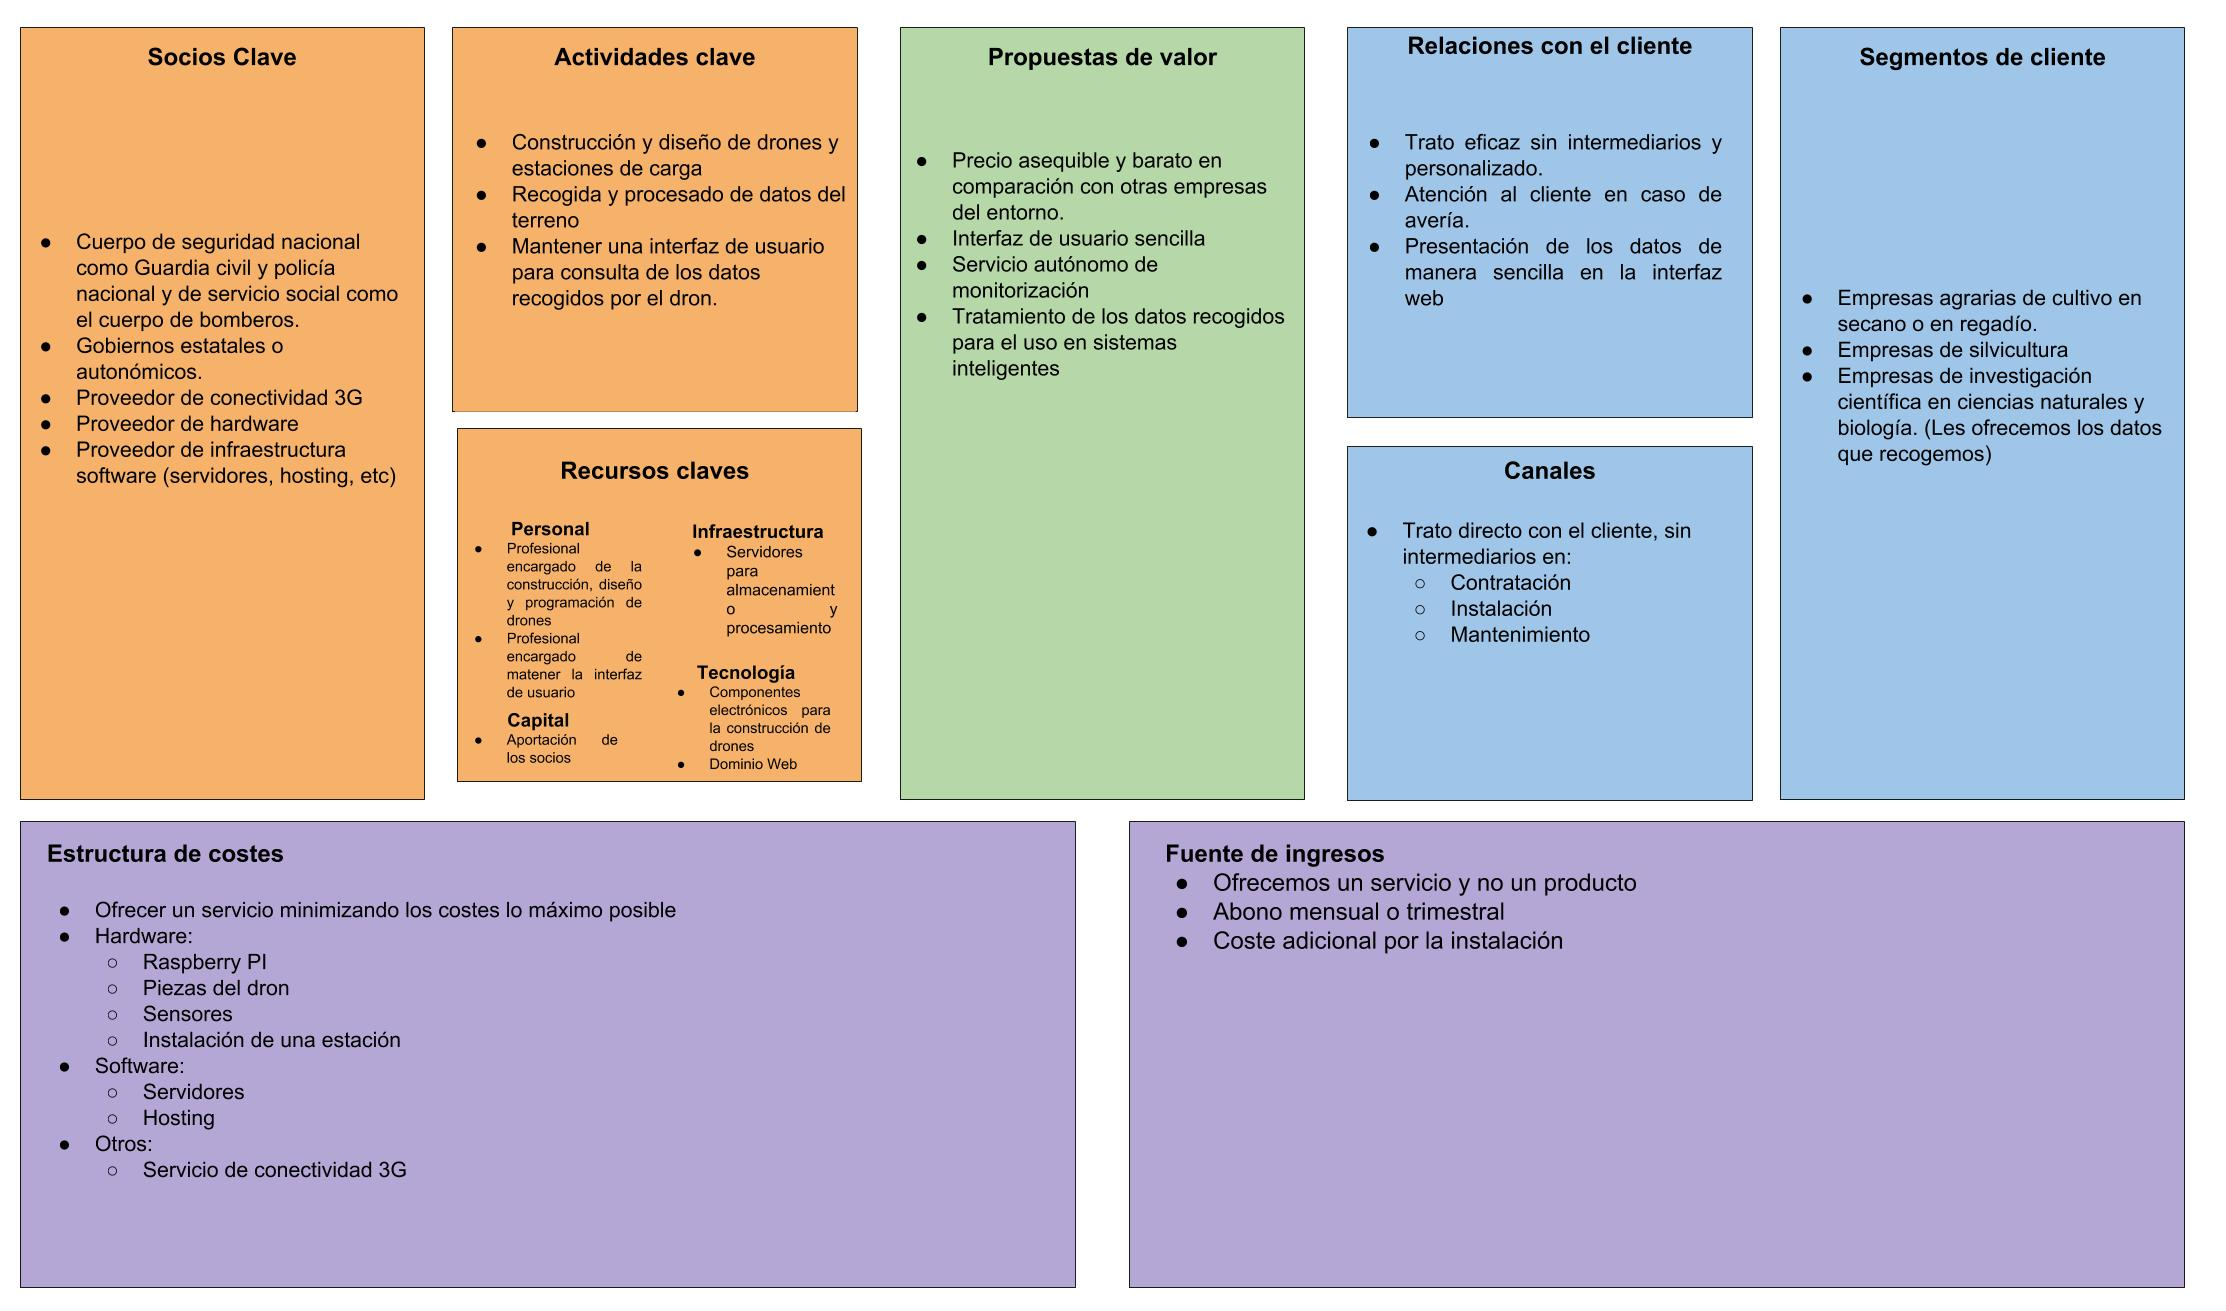
\includegraphics[totalheight=8cm]{img/modelo_de_negocio_canvas}
	\label{fig:business_model_canvas}
\end{figure}

\newpage

\section{Diseño inicial de la propuesta}

\subsection{¿En qué entorno se puede aplicar su producto?}
Aplicación directa en espacios naturales abiertos como campos de cultivo, bosques o grandes plantaciones. También resulta útil en reservas forestales, espacios protegidos y en general cualquier sitio con vegetación que se quiera monitorizar.


\subsection{Describa un ejemplo de caso de uso de su producto (cómo funcionaría desde el punto de vista del usuario)}

Acceso a una interfaz intuitiva que permite gestionar uno o más drones instalados con sus respectivas bases. La interfaz proporciona una imagen aérea de los cultivos y permite aplicar diferentes filtros en la interfaz para visualizar diferentes parámetros de cultivo. Existe una página principal que proporciona datos generales de dicho cultivo. A partir del análisis de dichos datos se generarán una serie de advertencias y/o sugerencias y una planificación de misiones para los drones. Dichas misiones pueden realizarse de forma autónoma cada cierto tiempo o activarse manualmente, según la preferencia del cliente.

\subsection{Describa brevemente qué elementos componen sus sistema, y qué función tienen}

\begin{figure}[H]
	\centering
	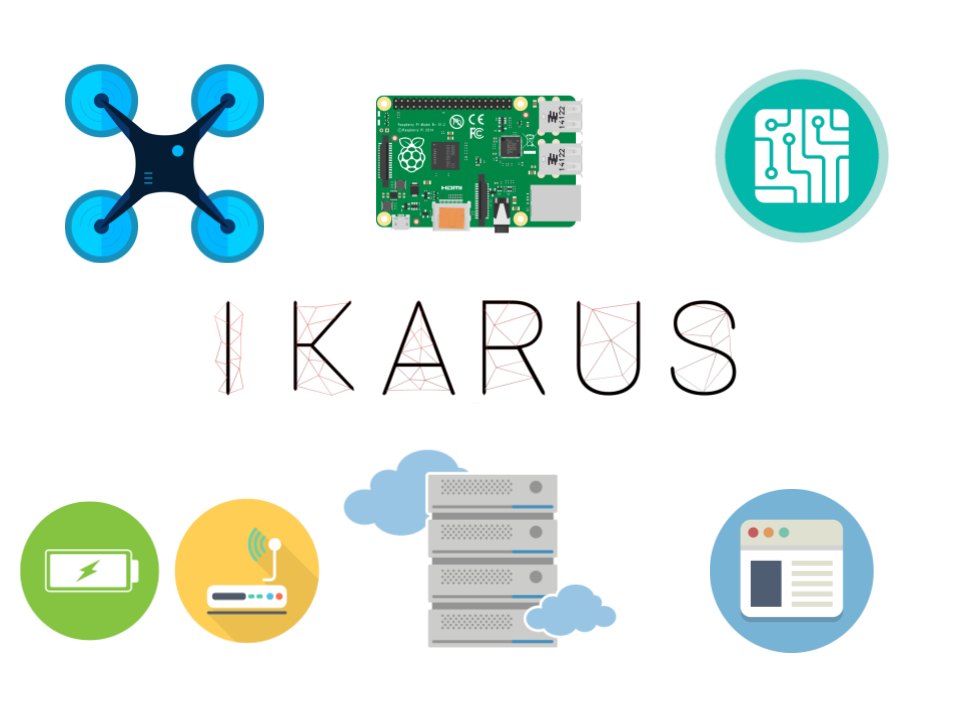
\includegraphics[totalheight=8cm]{img/componentes_ikarus.png}
	\caption{Componentes del sistema}
	\label{fig:esquema_inicial}
\end{figure}

Los 6 componentes de nuestro sistema (Figura \ref{fig:esquema_inicial}) son:
\begin{itemize}
\item \textbf{Dron Aéreo}: se encarga de volar de manera autónoma por la zona a monitorizar, llevando consigo la raspberry pi y los sensores.

\item \textbf{Raspberry Pi}: pequeño ordenador encargado de recoger los datos con sensores que lleva conectados.

\item \textbf{Sensores}: cámara multiespectral y térmica. 

\item \textbf{Estación}: base cubierta que sirve de resguardo al dron. Además, es el punto de envío de los datos recogidos a los servidores y carga de la batería del sistema de recolección de datos (dron, raspberry pi  y sensores)

\item \textbf{Servidores}: procesar y almacenar la información que ha sido enviada desde el lugar de monitorización.

\item \textbf{Interfaz web}: disponible para que el usuario pueda consultar los parámetros de interés sobre la monitorización de su terreno.
\end{itemize}

\subsection{Indique qué tecnología piensan usar para implementar los elementos del sistema.}
El software a utilizar será el código necesario para el control del cuadricóptero durante su vuelo usando una Raspberry Pi B+. La sección de hardware consistirá en el ensamblaje de los componentes individuales necesarios para el vuelo y la navegación así como usar Navio+ para pruebas. Los componentes no los seleccionaremos en un kit sino que lo haremos individualmente. La parte de toma de imágenes será llevada a cabo con una Raspberry Pi 3 y librerías de procesamiento de imágenes. Para el funcionamiento en conjunto del sistema usaremos RTI Connext DDS y será necesario realizar una interfaz web para el usuario.

% TODO: hacer

%%%%%%%%%%%%%%%%%%%%%%%%%%%%%%%%%%%%%%%%%%%%%%%%%%%%%%%%%%%%%%%%%%%%%%%%%%%%%%%%%%

% % % % % % % % % % % % % % % % % % % % % % % % % % % % % % % % %
%					 Bibliografía
% % % % % % % % % % % % % % % % % % % % % % % % % % % % % % % % 
\end{document}